\chapter{Means Comparison}\label{ch:mc}

\section{Methods}

\subsection{Introduction}
Bull run and Kingston power plants installed scrubbers in the year 2008 as mandated by the EPA.
These scrubbers may have significantly reduced the amount of sulfur dioxide emitted by the smoke stacks.
According to \autoref{fig:sulfateemissions}, which is a bar chart depicting the sum of sulfur dioxide emissions of Kingston and Bull run power plants,  the sulfur dioxide concentration dropped from 80 thousand tons in 2008 to about 15 thousand tons in 2009.
Interestingly the through fall SO$_4$ concentrations dramatically decline from about 115 $\mu$eq L$^{-1}$ in 2007 to about 30 $\mu$eq L$^{-1}$ in 2010.
\begin{figure}[h!]
  \centering
  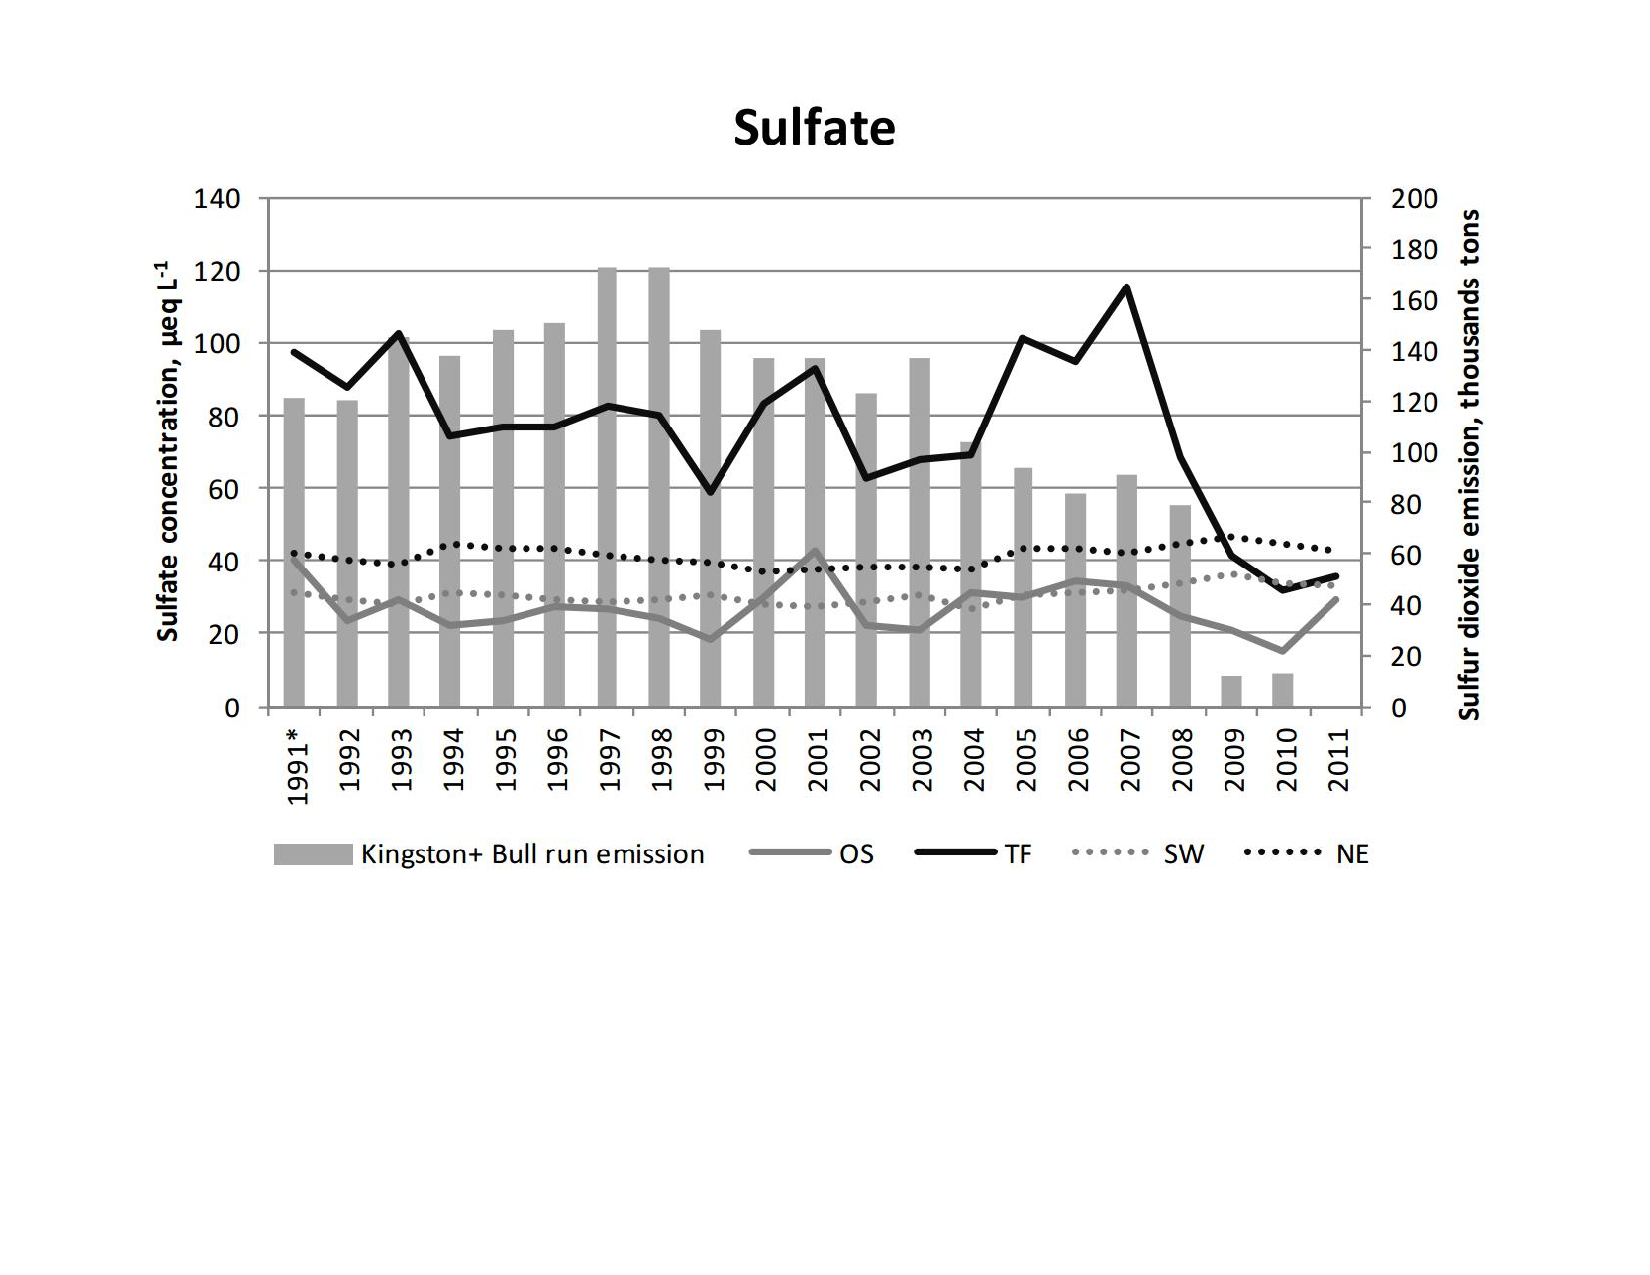
\includegraphics[width=6in]{SulfateEmissions}\\
  \caption{Sulfate emmisions of Kingstion and Bull run against those measured in Noland high elevation site \citep{annualreport2012}.}\label{fig:sulfateemissions}
\end{figure}
The hypothesis is that the decrease in sulfur dioxide emissions could correlate to the decrease in SO$_4$ concentrations measured in Noland Divide through fall.
And assuming that the sulfur dioxide emissions from Kingston and Bull run power plants affect the whole GRSM park then there may be signals for this affect in the data.
To examine this each time set will be tested against each other by way of means comparison methods.

\subsubsection{Instruments}
ANOVA is the standard means comparison method.
But it cannot compare more than two groups at once , and a method is needed that can compare all three time sets.
The Bonferroni multiple comparisons method is an option in the SPSS statistical program and can compare more than two groups at a time.
The explanation of the Bonferroni method given by the SPSS manual is that this method uses t tests to perform pairwise comparisons between group means and that the observed significance level is adjusted for the fact that multiple comparisons are being made \citep{spss}.

The Bonferroni method will create two specific types of outputs.
The first is a line graph showing the means of each group analyzed.
And the second is  a table of pairwise listings of all the groups compared to each other.
This table contains 95$\%$ confidence intervals and the significance associated with each comparison.
These confidence intervals are produced by the difference in means between the two groups being compared.
If the confidence interval includes zero then the groups are statistically the same or equal.

Using SPSS and the Bonferroni method three time sets (93-02, 03-08, 09-12) will be compared at six elevation class levels and across four water quality variables (pH, ANC, NO$_3$, and SO$_4 $).
Each group compared is the same stream survey data analyzed in chapter 2 and chapter 4 of this paper.

\section{Results}%probably shouldn't write so much on how the figures are misleading
\begin{table}[htbp]
\caption{Bonferroni comparisons between multiple groups}
\begin{center}
\begin{tabular}{p{2cm}cccccccccccc}
\toprule
 Elevation Classes& \multicolumn{ 3}{c}{pH} & \multicolumn{ 3}{c}{ANC} & \multicolumn{ 3}{c}{Nitrate} & \multicolumn{ 3}{c}{Sulfate} \\ \cline{2-13}\noalign{\smallskip}
 & \multicolumn{ 1}{c}{1-2} & 1-3 & 2-3 & 1-2 & 1-3 & 2-3 & 1-2 & 1-3 & 2-3 & 1-2 & 1-3 & 2-3 \\  \cline{2-13}
\multicolumn{1}{c}{1} & \textbf{$\neq$} & \textbf{$\neq$} & \textbf{$\neq$} & \textbf{=} & \textbf{=} & \textbf{=} & \textbf{$\neq$} & \textbf{=} & \textbf{=} & \textbf{=} & \textbf{=} & \textbf{=} \\ 
\multicolumn{1}{c}{2} & \textbf{=} & \textbf{=} & \textbf{=} & \textbf{=} & \textbf{$\neq$} & \textbf{=} & \textbf{$\neq$} & \textbf{$\neq$} & \textbf{=} & \textbf{$\neq$} & \textbf{$\neq$} & \textbf{=} \\ 
\multicolumn{1}{c}{3} & \textbf{$\neq$} & \textbf{$\neq$} & \textbf{$\neq$} & \textbf{=} & \textbf{$\neq$} & \textbf{=} & \textbf{=} & \textbf{$\neq$} & \textbf{$\neq$} & \textbf{=} & \textbf{=} & \textbf{=} \\ 
\multicolumn{1}{c}{4} & \textbf{=} & \textbf{$\neq$} & \textbf{$\neq$} & \textbf{=} & \textbf{=} & \textbf{=} & \textbf{=} & \textbf{=} & \textbf{=} & \textbf{=} & \textbf{=} & \textbf{=} \\ 
\multicolumn{1}{c}{5} & \textbf{$\neq$} & \textbf{$\neq$} & \textbf{$\neq$} & \textbf{=} & \textbf{$\neq$} & \textbf{$\neq$} & \textbf{$\neq$} & \textbf{=} & \textbf{$\neq$} & \textbf{=} & \textbf{=} & \textbf{=} \\ 
\multicolumn{1}{c}{6} & \textbf{=} & \textbf{$\neq$} & \textbf{$\neq$} & \textbf{=} & \textbf{=} & \textbf{=} & \textbf{=} & \textbf{=} & \textbf{=} & \textbf{=} & \textbf{=} & \textbf{=} \\ 
\bottomrule
\end{tabular}
\end{center}
\label{tab:Bontable}
\end{table}
\autoref{tab:Bontable} reports the Bonferoni comparison means between the four water quality variables (pH, ANC, NO$_3$, SO$_4$) in one time set against the same water quality variable in another time set by elevation bands.
In the table there are three columns per water quality variable.
And each column represents the comparison of two groups of the same variable in different times.
If the Bonferroni comparison found the groups to be equal then equality was represented by an equal sign.
If the groups are not equal an not equal sign was used to show this.
All groups that were found to be equal were insignificant and all groups that were unequal are significant at the 0.05 $\alpha$ level.
The bonferoni figures are presented in \autoref{app:bon}.
There are six figures for each of the water quality variables, one for each of the elevation classes.
For the most part the figures representing pH seem to be continuing a similar rate of change through the years, but this is also misleading because the time sets do not contain equal numbers of years.

The set comparisons between pH are the first comparisons presented.  
pH contains more unequal sets than any other water quality variable.
Mostly all the sets are different except between elevation class 2 which is all the same and class 4 and 6 which show sets 1 and 2 being equal.  
If a pronounced elevational trend existed for pH in the GRSM, this trend would be visible in the Bonferroni figures.
Following the means of each time set through the different elevation classes the largest mean should be in elevation class 1 and the smallest in elevation class 6.
Unfortunately elevation class 2 alway contains the lowest means instead of Elevation class 6.
And elevation class 3 behaves as if it should be between elevation class 5 and 6.

In contrast to the pH figures, the ANC figures do not all have similar rates of change.
In the odd numbered classes ANC reached a peak in set 2 and dropped for set 3.
All of the ANC figures have a decreasing trend from set 2 to 3 except for class 2 which is steadily increasing. 
The comparison found a lot of equality between the means of the ANC sets.  
Elevations 1, 4, and 6 are all equal.  
At elevations 2 and 3 set 1 and 3 are the only sets that are unequal. 
And at elevation 5 sets 1 and 2 are equal but set 3 is not.
The set means presented in the ANC figures vary greatly in concentration.
Classes and 1 and 2 are more than double the means of the other classes.
The ANC concentrations of elevation class 2 are the lowest which helps explain why the pH of elevation class 2 is also the lowest.
It is important to note here that even though class 2's concentrations are the lowest, they are also the only concentrations that are increasing.

For NO$_3$ elevation classes 4 and 6 are all the same and elevation 3 shows sets 1 and 2 being equal where 3 is not.  
Elevation class 1 is the opposite of expected showing all being equal except for sets 1 and 2.  
In elevation class 2 sets 3 and 2 are equal and in elevation class 5 sets 3 and 1 are equal.
The odd numbered figures for NO$_3$ all have decreasing mean values from set 2 to 3.
In elevation classes 2 and 4 the mean values for set 3 are higher than those in set 2 but the rate of increase is slowing.
Elevation 6 is always increasing.
The NO$_3$ figures show mostly decreasing concentrations over time, except for class 6.
The odd classes all have decreasing negative trends from set 2 to set 3 while classes 2 and 4 have decreasing positive trends between set 2 and 3.

SO$_4$ shows all three sets being equal across all elevation classes except for class 2.  
Class 2 shows only sets three and two being equal.
These figures can sometimes be misleading when visually comparing groups and it is always best to have the confidence intervals on hand.
For example when looking at the SO$_4$ figures many of the means look different across the time sets, but according to the table, except for class 2, they are all equal across time sets.
All of the set 3 means for SO$_4$ are larger than their respective set 2 means except for those in class 2 which has negative trends throughout.

\section{Discussion}
Because this analysis was completed after the trend analysis and descriptive statistics for these data sets were available certain results were expected.
Such as the increase in pH over time and the abnormal ANC concentrations.
The apparent decrease in ANC overtime as indicated in the Bonferroni figures was unexpected both because this is in contrast to the Julian date coefficients for ANC and pH has an increasing trend overtime.
Because the Bonferroni method calculates significant means for the water quality vector the difference between the figures and the trends suggests error in the trend analysis models.

The focus of this chapter was to investigate the decline in sulfur dioxide emissions from the Kingston and Bull run power plants and how it may impact the decline in SO$_4$  concentrations in the through fall measurements of the Noland divide high elevation site.
If a correlation existed it would be apparent in the pH results, but especially in the SO$_4$ results.
A significant negative difference in means for set 3 compared to sets 1 and 2 would support the hypothesis.
The inequalities present between the sets of pH data display a possible connection to the decline in sulfur dioxide pollution but there are many other factors that effect stream pH.
The comparisons between the SO$_4$ sets are unfortunately mostly equal.
This suggests a bank of SO$_4$ with a more steady output evidenced in the measured stream concentrations versus the quickly declining emissions measured as proposed input.
The pollution is taken in by the forest and slowly released into the streams.
More time may be needed to see affects of the scrubbers.
%sulfate sequestration?
